\documentclass[11pt]{article}
\usepackage[letterpaper,margin=1.02in]{geometry}
\usepackage[T1]{fontenc}
\usepackage{lmodern}
\usepackage{amsmath,amssymb,amsthm,booktabs,microtype}
\usepackage{tikz}
\usepackage[colorlinks=true,linkcolor=blue!40!black,urlcolor=blue!40!black,citecolor=blue!40!black]{hyperref}
\hypersetup{pdftitle={Autonomy Dimension of Graphs: Spectral Separation, Product Activation, and Entropy Bounds},
 pdfsubject={Separating vertices by autonomous binary observations of random walks},
 pdfkeywords={graph theory, random walks, lumpability, perfect colorings, entropy}}
\newtheorem{theorem}{Theorem}[section]
\newtheorem{lemma}[theorem]{Lemma}
\newtheorem{proposition}[theorem]{Proposition}
\newtheorem{corollary}[theorem]{Corollary}
\theoremstyle{definition}
\newtheorem{definition}[theorem]{Definition}
\newtheorem{remark}[theorem]{Remark}
\newcommand{\adim}{\operatorname{adim}}
\newcommand{\R}{\mathbb R}
\newcommand{\F}{\mathbb F}
\newcommand{\one}{\mathbf 1}
\newcommand{\HH}{H_2}
\newcommand{\Aut}{\mathcal A}
\numberwithin{equation}{section}
\setlength{\emergencystretch}{2em}
\raggedbottom
\title{Autonomy Dimension of Graphs:\\Spectral Separation, Product Activation,\\and Entropy Bounds}
\author{}
\date{October 7, 2026}

\begin{document}
\maketitle
\begin{abstract}
An autonomous binary coordinate on a graph is a two-coloring for which the
probability that a simple random walk changes color depends only on its
present color. We study the least number of such coordinates needed to
distinguish all vertices, called the autonomy dimension, with value infinity
when no separating family exists. We give a spectral criterion for
finiteness and prove two structural results. First,
$\adim(C_5)=\infty$ but $\adim(C_5\square C_5)=6$: taking a Cartesian
product can create a separating family even when neither factor has one.
Second, if $W_r$ consists of $r$ copies of $K_4$ sharing one vertex, then
\[
 \adim(W_r)=\frac{\log_2(3r)}{H_2(1/3)}+O(\log\log r).
\]
Thus exact autonomous observation has an asymptotic cost strictly above
the information bound for naming vertices. We also classify cycles,
establish a complement invariance for regular graphs, and show that finite
autonomy dimension is generically destroyed by arbitrary positive edge
weights. The elementary proofs are accompanied by exact finite checks.
Individual coordinates are classical binary strong lumpings; the proposed
organizing invariant is the minimum size of a separating family.
\end{abstract}

\noindent\textbf{Keywords.} Strong lumpability; perfect two-coloring;
graph spectrum; Cartesian product; separating family; binary entropy.

\section{Definition and purpose}

Throughout, $G=(V,E)$ is a finite connected simple undirected graph with
$n\geq2$ vertices, unless weights are explicitly introduced. Let $P$ be its
simple random walk operator,
\[
 (Pf)(v)=\frac{1}{\deg(v)}\sum_{w\sim v}f(w),
 \qquad \pi(v)=\frac{\deg(v)}{2|E|}.
\]
The question is whether a vertex can be described completely by a small
number of binary observations, each of which has closed Markov dynamics.

\begin{definition}\label{def:autonomy}
A nonconstant function $f:V\to\{0,1\}$ is \emph{autonomous} if there are
constants $a,b\in[0,1]$ such that
\[
 \frac{|\{w\sim v:f(w)\ne f(v)\}|}{\deg(v)}
 =\begin{cases}a,&f(v)=0,\\ b,&f(v)=1.\end{cases}
\]
The \emph{autonomy dimension} $\adim(G)$ is the least $d$ for which there
exist autonomous $f_1,\ldots,f_d$ making
$v\mapsto(f_1(v),\ldots,f_d(v))$ injective. If no such family exists,
set $\adim(G)=\infty$.
\end{definition}

For a simple random walk $(X_t)$, an autonomous $f$ makes $(f(X_t))$ a
Markov chain, for every initial distribution, with the same transition
matrix
\[
 \begin{pmatrix}1-a&a\\b&1-b\end{pmatrix}.
\]
Indeed, conditioning further on the current vertex does not change the
prescribed transition probabilities. Conversely, requiring this same
matrix for walks started at every vertex gives Definition~\ref{def:autonomy}
at the first step. Connectedness implies $a,b>0$.

Each coordinate therefore predicts its own next-step law from its current
value alone. Different coordinates need not be statistically independent,
and their joint transition law need not be a product law. Injectivity means
only that their simultaneous observations recover the vertex exactly.

An individual coordinate is a classical binary strong lumping; see
Geiger and Temmel~\cite{GT}. On a regular graph it is equivalently a perfect
two-coloring, or equitable two-partition, as studied in~\cite{BKM}.
The spectral and product constructions belong to the broader theory of
perfect structures~\cite{Taranenko}. We use these established objects to
ask a simultaneous separation question. The terminology and invariant are
proposed here as an organizing viewpoint; priority for the invariant or
the exact consequences below has not been established by a comprehensive
literature review. The mathematical claims are supported by the proofs,
independently of any claim of historical novelty.

\section{Spectral separation and elementary operations}

Write $\pi(f)=\sum_v\pi(v)f(v)$, and define
\[
 \Aut(G)=\operatorname{span}_{\R}
 \{f-\pi(f)\one:f\text{ is autonomous}\}.
\]
The zero space is allowed. A space of functions \emph{separates vertices}
if, for every $u\ne v$, at least one function in the space has different
values at $u$ and $v$.

\begin{theorem}[Spectral separation]\label{thm:spectral}
An autonomous binary $f$ with parameters $(a,b)$ satisfies
\begin{equation}\label{eq:eigen}
 P\left(f-\frac{a}{a+b}\one\right)
 =(1-a-b)\left(f-\frac{a}{a+b}\one\right),
 \qquad \pi(f)=\frac{a}{a+b}.
\end{equation}
Conversely, every real eigenvector of $P$ with exactly two values is an
affine rescaling of an autonomous binary function. In particular,
$\adim(G)<\infty$ if and only if the two-valued real eigenvectors separate
all vertices. Whenever the dimension is finite,
\begin{equation}\label{eq:bounds}
 \lceil\log_2 n\rceil\leq\adim(G)
 \leq\dim\Aut(G)\leq n-1.
\end{equation}
\end{theorem}

\begin{proof}
The defining condition is exactly
$Pf=a\one+(1-a-b)f$. Applying the stationary functional $\pi$ gives
$(a+b)\pi(f)=a$, proving~\eqref{eq:eigen}.

Conversely, normalize the two values of an eigenvector to $0$ and $1$,
obtaining a nonconstant binary $f$. The eigenvector equation says that
$Pf$ is an affine function of $f$, hence constant on each of its two
classes. Its value on class $0$ is the cross-class probability $a$; its
value on class $1$ is $1-b$. Thus $f$ is autonomous.

The family of generators of $\Aut(G)$ separates vertices if and only if
its span does. If it separates, choose a basis from these generators.
Equality of all basis values at two vertices would force equality of
every value in the span. The corresponding binary coordinates therefore
separate, proving the middle bound. Every generator has stationary mean
zero, so the space has dimension at most $n-1$. Finally, $d$ binary
coordinates have at most $2^d$ different codes.
\end{proof}

\begin{corollary}[Integer spectral obstruction]\label{cor:integer}
If $G$ is $q$-regular, every autonomous binary coordinate gives an integer
adjacency eigenvalue other than $q$. Consequently, if the adjacency matrix
has no integer eigenvalue other than $q$, then $\adim(G)=\infty$.
\end{corollary}

\begin{proof}
The numbers of opposite-color neighbors are integers $c_0=qa$ and
$c_1=qb$. The centered coordinate has adjacency eigenvalue
$q-c_0-c_1$, which is an integer and is smaller than $q$ since $a,b>0$.
\end{proof}

The obstruction immediately gives $\adim(C_5)=\infty$: the nonprincipal
adjacency eigenvalues are $(\sqrt5-1)/2$ and $-(\sqrt5+1)/2$, each twice.
At the other extreme, every nonconstant binary function on $K_n$ is
autonomous, so
\begin{equation}\label{eq:basic}
 \adim(K_n)=\lceil\log_2 n\rceil,\qquad \adim(Q_d)=d\quad(d\geq1).
\end{equation}
For the cube, its usual coordinate bits are autonomous with $a=b=1/d$;
the information bound proves optimality.

\begin{proposition}[Complement and product laws]\label{prop:operations}
If both $G$ and $\overline G$ are connected regular graphs, then
$\adim(G)=\adim(\overline G)$. If $G,H$ are connected regular graphs and
both autonomy dimensions are finite, then
\[
 \adim(G\square H)\leq\adim(G)+\adim(H).
\]
\end{proposition}

\begin{proof}
For a fixed binary partition of a regular graph, autonomy is equivalent
to a constant number of opposite-color neighbors within each class.
In the complement that number becomes the size of the opposite class
minus its original value. Thus the two graphs have exactly the same
autonomous binary functions.

If $G,H$ have degrees $q,s$, respectively, lift a coordinate of $G$ to
$(x,y)\mapsto f(x)$. Its two flip probabilities are multiplied by
$q/(q+s)$ on the Cartesian product, so it remains autonomous. Coordinates
of $H$ lift in the same way with factor $s/(q+s)$. Combining separating
families from both factors separates the product.
\end{proof}

There is also a finite exact procedure. Enumerate the nonconstant binary
functions up to complementation, retain the autonomous ones, and associate
to each the unordered vertex pairs that it separates. If some pair is
uncovered, the dimension is infinite. Otherwise the dimension is the
minimum number of these sets covering all pairs. This is an exact finite
set-cover formulation, not a claim of an efficient algorithm or a
complexity hardness result.

\section{An asymptotically sharp cost of autonomy}

Let $W_r$ be the graph obtained from $r$ copies of $K_4$ by identifying one
vertex of each copy to a common hub $o$. Removing $o$ leaves $r$ disjoint
triangles. There are $3r+1$ vertices; the hub has degree $3r$ and each
outer vertex has degree $3$.

For $0\leq p\leq1$, put
\[
 \HH(p)=-p\log_2 p-(1-p)\log_2(1-p),\qquad
 h=\HH(1/3)=\log_2 3-\frac23,
\]
with $0\log_2 0=0$. Numerically, $h=0.918295834\ldots$.

\begin{theorem}[Sharp asymptotic overhead]\label{thm:windmill}
For every integer $r\geq1$, the autonomy dimension of $W_r$ is finite and
\begin{equation}\label{eq:windmillbounds}
 \left\lceil\frac{\log_2(3r)}{h}\right\rceil
 \leq\adim(W_r)
 \leq\min\left\{3k:k\geq1,\ \binom{3k}{k}\geq9r\right\}.
\end{equation}
Consequently, as $r\to\infty$,
\begin{align}
 \adim(W_r)&=\frac{\log_2(3r)}{h}+O(\log\log r),\label{eq:windasymp}\\
 \frac{\adim(W_r)}{\log_2|V(W_r)|}&\longrightarrow
 \frac1h=1.088973686\ldots.\label{eq:windratio}
\end{align}
In particular, $\adim(W_r)-\lceil\log_2|V(W_r)|\rceil$ tends to infinity.
\end{theorem}

\begin{lemma}[Coordinates on the windmill]\label{lem:windcuts}
Orient an autonomous binary coordinate so that $f(o)=0$. Its class $1$
consists of exactly $k$ vertices from each outer triangle, for one common
$k\in\{1,2,3\}$. Conversely, every such choice is autonomous, with
\[
 a=k/3,\qquad b=(4-k)/3.
\]
\end{lemma}

\begin{proof}
Some outer vertex is selected because the function is nonconstant.
The hub therefore has positive flip probability. If a triangle had no
selected vertex, its zero vertices would have flip probability zero,
a contradiction. Let $k_i\geq1$ be the number selected in triangle $i$.
A selected vertex there has $4-k_i$ zero neighbors, including the hub,
out of degree $3$. Constancy on selected vertices forces all $k_i$ to
agree. Conversely, if they all equal $k$, the hub has flip probability
$rk/(3r)=k/3$, every outer zero has $k$ selected neighbors, and every
selected vertex has $4-k$ zero neighbors. When $k=3$ the hub is the only
zero vertex, so the same formulas still hold.
\end{proof}

\begin{lemma}[Entropy obstruction]\label{lem:entropy}
Let $Z$ have any probability distribution on the vertices of a graph.
If every autonomous binary $f$ satisfies $H(f(Z))\leq\eta$, then every
separating family of $d$ autonomous coordinates satisfies
$H(Z)\leq d\eta$, where entropies are in bits.
\end{lemma}

\begin{proof}
Injectivity gives $H(Z)=H(f_1(Z),\ldots,f_d(Z))$. The entropy chain rule
and the fact that conditioning cannot increase entropy give
$H(f_1(Z),\ldots,f_d(Z))\leq\sum_j H(f_j(Z))\leq d\eta$.
No independence assumption is used.
\end{proof}

\begin{proof}[Proof of Theorem~\ref{thm:windmill}]
Choose $Z$ uniformly among the $3r$ outer vertices. After complementing
any coordinate if necessary, Lemma~\ref{lem:windcuts} gives
$\Pr(f(Z)=1)\in\{1/3,2/3,1\}$. Hence $H(f(Z))\leq h$, and
Lemma~\ref{lem:entropy} proves the lower bound.

For the upper bound, fix $k\geq1$. Form a hypergraph whose vertices are
the $k$-element subsets of $[3k]$ and whose hyperedges are the unordered
partitions of $[3k]$ into three such subsets. It has
\[
 B=\binom{3k}{k}\quad\text{vertices},\qquad
 \Delta=\frac12\binom{2k}{k}\quad\text{edges through each vertex},
\]
and therefore $B\Delta/3$ hyperedges. Take a maximal matching $M$ of
pairwise vertex-disjoint hyperedges. Every hyperedge meets a member of
$M$, while each member meets at most $3\Delta$ hyperedges. Thus
\[
 \frac{B\Delta}{3}\leq3\Delta|M|,
 \qquad |M|\geq\frac B9.
\]
If $B\geq9r$, select $r$ of these partitions. In triangle $i$, assign the
three incidence words of the three blocks of partition $i$, and assign
the all-zero word to the hub. All $3r$ outer words are distinct because
the hyperedges are disjoint as sets of blocks; each word is nonzero.
Every coordinate selects exactly one vertex per triangle. By
Lemma~\ref{lem:windcuts}, every coordinate is autonomous. This gives a
separating code of length $3k$ and proves finiteness and the upper bound.

Stirling's formula gives
\[
 \log_2\binom{3k}{k}=3kh-\tfrac12\log_2 k+O(1).
\]
For $L=\log_2(3r)$, choosing
$k=\lceil(L+\log_2 L+C)/(3h)\rceil$ with a fixed sufficiently large $C$
makes $\binom{3k}{k}\geq9r$ for all sufficiently large $r$.
The upper bound is therefore $L/h+O(\log L)$, which together with the
lower bound proves~\eqref{eq:windasymp}. The ratio follows since
$\log_2(3r+1)=\log_2(3r)+o(1)$. Finally $1/h>1$, so even the lower bound
exceeds $\lceil\log_2(3r+1)\rceil$ by a quantity tending to infinity.
\end{proof}

The coefficient in~\eqref{eq:windratio} identifies a quantitative cost:
the allowed coordinates convey at most $h<1$ bit each under a natural
vertex distribution. The construction shows that this entropy cost is
asymptotically attainable. Thus autonomy dimension contains information
that the order of a graph alone cannot express.

\begin{proposition}[The smallest windmill obstruction]\label{prop:w2}
For two copies of $K_4$ sharing a vertex, $\adim(W_2)=4$, although
$\lceil\log_2 7\rceil=3$.
\end{proposition}

\begin{proof}
Suppose that three coordinates suffice, and complement them to make the
hub $000$. The six outer vertices then receive six distinct nonzero
three-bit words. There are seven such words, so exactly one nonzero word
$w$ is omitted. In each column, Lemma~\ref{lem:windcuts} requires equally
many ones in the two triangles, hence an even total. But all seven
nonzero words contain four ones in each column, so removing any nonzero
$w$ leaves an odd total in a column where $w$ is one. This is impossible.

For a four-coordinate construction use hub $0000$, and assign the words
\[
 \{1000,0100,0011\},\qquad \{0010,0001,1100\}
\]
to the two triangles. Each column selects exactly one vertex of each
triangle, and all seven words are distinct.
\end{proof}

\begin{figure}[ht]
\centering
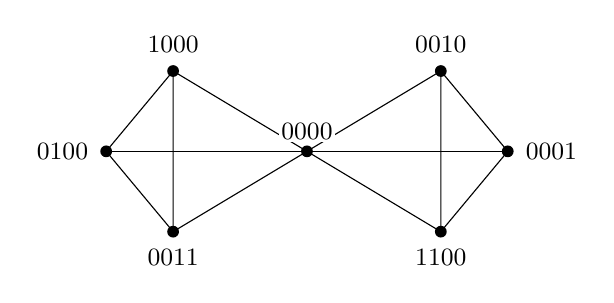
\begin{tikzpicture}[scale=0.85,every node/.style={font=\small}]
 \coordinate (o) at (0,0);
 \coordinate (a) at (-2,1.2); \coordinate (b) at (-3,0);
 \coordinate (c) at (-2,-1.2);
 \coordinate (d) at (2,1.2); \coordinate (e) at (3,0);
 \coordinate (f) at (2,-1.2);
 \draw (a)--(b)--(c)--(a) (d)--(e)--(f)--(d);
 \foreach \x in {a,b,c,d,e,f}{\draw (o)--(\x);}
 \foreach \x in {o,a,b,c,d,e,f}{\fill (\x) circle (2.5pt);}
 \node[above=3pt,fill=white,inner sep=1pt] at (o) {$0000$};
 \node[above=3pt] at (a) {$1000$};
 \node[left=3pt] at (b) {$0100$};
 \node[below=3pt] at (c) {$0011$};
 \node[above=3pt] at (d) {$0010$};
 \node[right=3pt] at (e) {$0001$};
 \node[below=3pt] at (f) {$1100$};
\end{tikzpicture}
\caption{An optimal autonomous code for $W_2$. Each column has flip
probabilities $a=1/3$ and $b=1$. Four coordinates are necessary.}
\end{figure}

\section{A product can create finite autonomy dimension}

The product bound of Proposition~\ref{prop:operations} does not have a
converse: the product can have finite dimension even if both factors have
infinite dimension.

\begin{theorem}[Product activation]\label{thm:product}
For the Cartesian product of two five-cycles,
\[
 \adim(C_5)=\infty,\qquad \adim(C_5\square C_5)=6.
\]
More precisely, writing its vertices as $(x,y)\in\F_5^2$, every autonomous
binary coordinate depends solely on one of the two quantities
\begin{equation}\label{eq:uv}
 u=x+2y\pmod5,\qquad v=x-2y\pmod5.
\end{equation}
Conversely, every nonconstant binary function of either quantity is
autonomous.
\end{theorem}

\begin{proof}
The assertion about $C_5$ follows from Corollary~\ref{cor:integer}.
On the Cartesian product, the four steps $(\pm1,0),(0,\pm1)$ change $u$
by $\pm1,\pm2$, each with probability $1/4$. They therefore send $u$ to
each of its other four values uniformly. The same holds for $v$. Each
projection has the transition law of simple random walk on $K_5$.
All binary partitions of $K_5$ are autonomous, proving the converse
claim. The transformation~\eqref{eq:uv} is invertible over $\F_5$ because
its determinant is $-4\ne0$. Encoding $u$ with three bits and $v$ with
three more therefore gives an injective autonomous six-bit code.

To prove optimality we classify all possible coordinates. Put
$\alpha=(\sqrt5-1)/2$ and $\beta=-(\sqrt5+1)/2$. The adjacency spectrum
of $C_5$ is $2,\alpha,\alpha,\beta,\beta$. The Cartesian adjacency
matrix is $A\otimes I+I\otimes A$; tensor products of eigenvectors give
all pairwise eigenvalue sums. Thus the product spectrum is
\[
 \begin{array}{c|rrrrrr}
 \text{eigenvalue}&4&2+\alpha&2+\beta&2\alpha&2\beta&-1\\
 \text{multiplicity}&1&4&4&4&4&8.
 \end{array}
\]
The only integer nonprincipal eigenvalue is $-1$. By
Corollary~\ref{cor:integer}, the centered version of every autonomous
coordinate lies in its eight-dimensional eigenspace.

Every mean-zero function of $u$ is a $-1$ adjacency eigenvector: the
sum over neighbors is the sum over the four other $u$-values, which is
the negative of the current value. These functions form a four-dimensional
space. The same is true for $v$, and the spaces have zero intersection,
because $(u,v)$ ranges over all of $\F_5^2$. Together they exhaust the
$-1$ eigenspace. Hence an autonomous binary $f$ has the form
\[
 f(x,y)=A(u)+B(v),
\]
where a constant can be absorbed into $A$.

If both $A$ and $B$ were nonconstant, choose values
$A_-<A_+$ and $B_-<B_+$. The three distinct sums
$A_-+B_-<A_-+B_+<A_++B_+$ all occur, contradicting the fact that $f$
has only two values. Thus $f$ depends on only one of $u,v$.

For any fixed $v$, the five possible $u$-values can only be separated by
the coordinates depending on $u$, of which at least three are required.
Likewise at least three coordinates depending on $v$ are necessary.
A nonconstant coordinate cannot depend solely on both, so these counts
add, giving the lower bound six.
\end{proof}

The graph has only 25 vertices, so its unconstrained binary labeling cost
is five. The sixth coordinate is forced by the two separate five-valued
observables. At the same time, neither original cycle admits even one
nonconstant autonomous coordinate. The phenomenon is therefore not
explained by simply lifting coordinates from the factors.

\section{Exact classification of cycles}

\begin{theorem}\label{thm:cycles}
For $n\geq3$,
\[
 \adim(C_n)=
 \begin{cases}
 2,&n=3,4,\\
 3,&n=6,\\
 4,&n=12,\\
 \infty,&\text{otherwise}.
 \end{cases}
\]
In fact, all autonomous binary coordinates together identify vertices
$i,j\in\mathbb Z/n\mathbb Z$ exactly when
$i\equiv j\pmod{\gcd(n,12)}$.
\end{theorem}

\begin{proof}
For each color $b$, the constant number $c_b$ of opposite-color neighbors
is either one or two. If $(c_0,c_1)=(2,2)$, the colors alternate with
period two. If $(c_0,c_1)=(1,2)$, every one is isolated and every zero
has exactly one zero neighbor, so every zero run has length two; the
pattern is a rotation of repeated $001$. The reversed pair is its
complement. If $(c_0,c_1)=(1,1)$, every run has length two and the pattern
is a rotation of repeated $0011$. These exhaust all possibilities, with
each period required to divide $n$.

The period-two patterns distinguish residues modulo two. All rotations
of the period-three patterns distinguish residues modulo three, and all
rotations of the period-four patterns distinguish residues modulo four.
Together, the available patterns distinguish residues modulo the least
common multiple of the available periods in $\{2,3,4\}$, taking this to
be one if none is available. This least common multiple is $\gcd(n,12)$.
Thus separation is possible exactly for $n=3,4,6,12$.

For these four sizes, the information bound gives the stated lower
bounds. For $C_3$, use any two different singleton indicators. For
$C_4$, use the two rotated patterns with codes $00,01,11,10$ in cyclic
order. For $C_6$, use parity and two singleton indicators modulo three.
For $C_{12}$, use two singleton indicators modulo three and two rotated
period-four patterns. The residue pairs separate by the Chinese remainder
theorem, giving the required numbers of coordinates.
\end{proof}

\section{The scope of exact autonomy}

The preceding results exploit exact equalities of transition probabilities.
The next theorem makes this limitation precise. Give each edge $e$ a
positive symmetric weight $w_e$, and use transition probabilities
$P_w(x,y)=w_{xy}/\sum_{z\sim x}w_{xz}$. Definition~\ref{def:autonomy}
then uses weighted cross-edge fractions.

\begin{theorem}[Generic weight obstruction]\label{thm:weights}
Fix a connected simple support graph with $n\geq3$. For Lebesgue-almost
every vector of positive edge weights, the weighted walk has infinite
autonomy dimension. More precisely, outside a set of measure zero, a
nonbipartite support has no nonconstant autonomous binary coordinate,
and a bipartite support has only its proper bipartition, up to complement.
\end{theorem}

\begin{proof}
Fix a nonconstant binary partition that is not a proper coloring. Some
monochromatic connected component has at least two vertices. Since the
whole graph is connected and both colors occur, that component contains
a boundary vertex $x$ with a neighbor $z$ of the opposite color. It also
contains a same-color neighbor of $x$. Choose any other vertex $y$ in the
component, so $x$ and $y$ have the same color.

Keep all weights except $w_{xz}=t$ fixed. The cross-color probability at
$x$ is $(t+C)/(t+C+D)$ with $D>0$, hence is strictly increasing in $t$.
The corresponding probability at $y$ does not depend on $t$. Equality of
these two probabilities, which autonomy requires, becomes a nonzero
polynomial equation in the edge weights after clearing the positive
denominators. Its solution set has Lebesgue measure zero. There are only
finitely many binary partitions, so the union of the exceptional sets
for all nonproper partitions still has measure zero.

A proper binary coloring always has both flip probabilities one.
A connected graph has such a coloring exactly when it is bipartite,
and then the coloring is unique up to complement. A single binary
partition cannot separate $n\geq3$ vertices. The result follows.
\end{proof}

This theorem does not contradict stability under a common rescaling of all
edge weights, or under symmetry-preserving changes. It concerns arbitrary
variation in the full positive edge-weight space. Exact autonomy dimension
measures exact organization of a transition law; an approximate version
would require a separate definition and separate theorems.

\section{Finite verification and further questions}

The companion program \texttt{verify\_autonomy\_dimension.py} uses integer
cross-multiplication to enumerate all autonomous cuts up to complement,
and an exact minimum set-cover search to calculate finite dimensions.
It uses NetworkX for graph generation and rational arithmetic for ranks.
The results are stored in \texttt{autonomy\_verification\_results.json}.
Running the script with Python and NetworkX reproduces the following checks.

\begin{table}[ht]
\centering
\begin{tabular}{rrrrrr}
\toprule
Order & Connected graphs & $\adim=1$ & $\adim=2$ & $\adim=3$ & $\adim=4$\\
\midrule
2&1&1&0&0&0\\
3&2&0&1&0&0\\
4&6&0&3&0&0\\
5&21&0&0&2&0\\
6&112&0&0&7&0\\
7&853&0&0&3&2\\
\bottomrule
\end{tabular}
\caption{Exact enumeration of the 995 connected unlabeled graphs on two
through seven vertices. The 19 graphs counted in the dimension columns
have finite dimension; all other 976 have infinite dimension.}
\end{table}

The checks also verify the spectral upper bound and regular complement
invariance on the applicable graphs in this range; exhaust all binary
cuts on $C_n$ for $3\leq n\leq18$; and confirm dimensions $2,4,4$ for
$W_1,W_2,W_3$. For $C_5\square C_5$, exact rational rank calculations
verify the eight-dimensional $-1$ eigenspace and the absence of other
nonprincipal integer eigenvalues. A minimum set-cover search on the
30 cuts classified in Theorem~\ref{thm:product} returns six. This last
enumeration uses the proved classification; it is not an exhaustive
search over all binary functions on 25 vertices.

Finally, the greedy matching construction in the proof of
Theorem~\ref{thm:windmill}, with $k=1,2,3,4$, produces separating codes
of lengths $3,6,9,12$ for $W_1,W_5,W_{25},W_{156}$, respectively.
All coordinate transition probabilities and code injectivity are checked
exactly. These finite checks supplement the proofs; they do not establish
the asymptotic or measure-theoretic statements.

The theory suggests several specific questions. Determine $\adim(W_r)$
exactly, beyond the asymptotic formula. Characterize the pairs of regular
graphs with infinite factor dimensions and finite product dimension.
Find efficient recognition algorithms for graph classes with few distinct
eigenvalues. For an approximate theory, one could bound the variation of
cross-color probabilities within each class and ask how the minimum
separating family changes with the tolerance. These questions concern a
well-defined invariant with spectral obstructions, explicit constructions,
and a sharp asymptotic separation from ordinary binary labeling.

\begin{thebibliography}{9}
\bibitem{BKM}
E.~A. Bespalov, D.~S. Krotov, A.~A. Matiushev, A.~A. Taranenko,
and K.~V. Vorob'ev,
\emph{Perfect $2$-colorings of Hamming graphs},
Journal of Combinatorial Designs \textbf{29} (2021), 367--396.
\href{https://arxiv.org/abs/1911.13151}{arXiv:1911.13151}.

\bibitem{GT}
B.~C. Geiger and C.~Temmel,
\emph{Lumpings of Markov chains, entropy rate preservation, and
higher-order lumpability},
\href{https://arxiv.org/abs/1212.4375}{arXiv:1212.4375}.

\bibitem{Taranenko}
A.~A. Taranenko,
\emph{Algebraic properties of perfect structures},
\href{https://arxiv.org/abs/1906.10430}{arXiv:1906.10430}.
\end{thebibliography}
\end{document}
